\documentclass[10pt,mathserif]{beamer}
\usepackage[english]{babel}
\usepackage[utf8]{inputenc}
\usepackage[T1]{fontenc}
\usepackage{cmbright}
\usepackage{tikz}
\usepackage{listings}
\usepackage{relsize}
\usepackage{booktabs}

\usetikzlibrary{automata}
\usetikzlibrary{positioning}
\usetikzlibrary{shapes.multipart}

\usetheme{Warsaw}
\useoutertheme{essential}
\setbeamertemplate{navigation symbols}{}

\author{Stefano Cherubin}
\institute{Politecnico di Milano}
\date{06-05-2016}
\title{Exploring LLVM}
\newcommand{\customdata}{Stefano Cherubin <stefano.cherubin@polimi.it>}
\renewcommand{\ttdefault}{pxtt}
\lstset{basicstyle=\ttfamily\scriptsize}
\newcommand{\cinput}[1]{\lstinputlisting[language=C]{#1}}
\newcommand{\cinline}[1]{\lstinline[language=C]!#1!}
\newcommand{\cppinput}[1]{\lstinputlisting[language=C++]{#1}}
\newcommand{\cppinline}[1]{\lstinline[language=C++]!#1!}
\newcommand{\llvminput}[1]{\lstinputlisting[language=LLVM]{#1}}
\newcommand{\llvminline}[1]{\lstinline[language=LLVM]!#1!}
\lstdefinelanguage{LLVM}%
  {morekeywords={define,declare,global,constant,internal,external,private,%
      linkonce,linkonce_odr,weak,weak_odr,appending,common,extern_weak,%
      thread_local,dllimport,dllexport,hidden,protected,default,except,deplibs,%
      volatile,fastcc,coldcc,cc,ccc,x86_stdcallcc,x86_fastcallcc,ptx_kernel,%
      ptx_device,signext,zeroext,inreg,sret,nounwind,noreturn,nocapture,byval,%
      nest,readnone,readonly,noalias,uwtable,inlinehint,noinline,alwaysinline,%
      optsize,ssp,sspreq,noredzone,noimplicitfloat,naked,alignstack,module,asm,%
      align,tail,to,addrspace,section,alias,sideeffect,c,gc,target,datalayout,%
      triple,blockaddress},%
  morekeywords=[2]{add,fadd,sub,fsub,mul,fmul,sdiv,udiv,fdiv,srem,urem,frem,%
     and,or,xor,icmp,fcmp,eq,ne,ugt,uge,ult,ule,sgt,sge,slt,sle,oeq,ogt,oge,%
     olt,ole,one,ord,ueq,ugt,uge,ult,ule,une,uno,nuw,nsw,exact,inbounds,phi,%
     call,select,shl,lshr,ashr,va_arg,trunc,zext,sext,fptrunc,fpext,fptoui,%
     fptosi,uitofp,sitofp,ptrtoint,inttoptr,bitcast,ret,br,indirectbr,switch,%
     invoke,unwind,unreachable,malloc,alloca,free,load,store,getelementptr,%
     extractelement,insertelement,shufflevector,extractvalue,insertvalue},%
  sensitive=t,%
  morestring=[b]",%
  morecomment=[l];%
  }[keywords,comments,strings]

\AtBeginSection[]
{
\begin{frame}{Contents}
\tableofcontents[currentsection]
\end{frame}
}
\begin{document}

\begin{frame}
\maketitle
\begin{center}
\itshape\scriptsize This material is strongly based on material produced by
                    Michele Scandale and Ettore Speziale for the course
                    `Code Optimizations and Transformations`.
\end{center}
\end{frame}

\section{Documentation}
\begin{frame}[t]{LLVM official documentation}
  \begin{center}
    \begin{Huge}
      \vfill
      \url{llvm.org/docs}
      \vfill
    \end{Huge}
  \end{center}
\end{frame}
%--- Next Frame ---%

\begin{frame}[t]{A lot of documentation...}
  \url{llvm.org/docs} mentions:
  \begin{itemize}
    \item \texttt{\ 5} references about \textit{Design \& Overview}
    \item \texttt{19} references about \textit{User Guides}
    \item \texttt{13} references about \textit{Programming Documentation}
    \item \texttt{32} references about \textit{Subsystem Documentation}
    \item \texttt{\ 7} references about \textit{Development Process Documentation}
    \item \texttt{\ 5} Mailing Lists
    \item \texttt{\ 5} IRC bots
  \end{itemize}
  \vfill
  Most of the above references are OUT-OF-DATE.
  \vfill
  You probably need documentation about the documentation itself.
  \vfill
\end{frame}
%--- Next Frame ---%

\begin{frame}[t]{Essential documentation}
  \begin{description}
    \item[Intro to LLVM] \cite{LOCAL:www/llvmIntro}
          gives a quick and clear introduction to the compiler infrastructure.
          It is mostly up-to-date.\footnote{at the time I am writing}
    \vfill
    \item[Writing an LLVM pass] \cite{LOCAL:www/llvmWritingAPass}
          explains step by step how to implement a Pass
          for those who never did anything like that.
          We will see this tutorial later in the course.
    \vfill
    \item[Doxygen] \cite{LOCAL:www/llvmDoxygen}
          \textit{The best code documentation is the code itself.}
          Sometimes the generated doxygen documentation is enough.
          It also contains links to the web version of the source code.
          It is always up-to-date.
    \vfill
    \item[llvm-dev] Mailing List. Last resource: ask other developers.
          Warning: 24/7 many people are posting in this ML.
  \end{description}
\end{frame}

\section{Normalization Passes}
\begin{frame}{Canonicalize Pass Input}
We will see the following passes:

\begin{table}
\centering
\begin{tabular}{cc}
\toprule

\multicolumn{1}{c}{\textbf{Pass}}    &
\multicolumn{1}{c}{\textbf{Switch}} \\

\midrule

Variable promotion  &
\texttt{mem2reg}   \\

Loop simplify           &
\texttt{loop-simplify} \\

Loop-closed SSA  &
\texttt{lcssa}  \\

Induction variable simplification  &
\texttt{indvars}                  \\

\bottomrule
\end{tabular}
\end{table}

They are \alert{normalization} passes:

\begin{itemize}
\item put data into a canonical form
\end{itemize}
\end{frame}

\begin{frame}{Variable Promotion}
One of the most difficult things in compiler is:

\begin{itemize}
\item considering memory accesses
\end{itemize}

\begin{block}{Plain SAXPY}
\centering
\llvminput{snippet/02/plain-saxpy.ll}
\end{block}
\end{frame}

\begin{frame}{Variable Promotion}{Simplifying Representation}
In the SAXPY kernel some \llvminline{alloca} are generated:

\begin{itemize}
\item represent \alert{local variables}~\footnote{Arguments are local variables}
\end{itemize}

They are generated due to compiler \alert{conservative} approach:

\begin{itemize}
\item maybe some instruction can take the addresses of such variables, hence a
      memory location is needed
\end{itemize}

Complex representations makes hard performing further actions:

\begin{itemize}
\item suppose you want to compute \cinline{a * x + y} using only one
      instruction~\footnote{e.g. FMA4}
\item hard to detect due to \llvminline{load} and \llvminline{store}
\end{itemize}
\end{frame}

\begin{frame}{Variable Promotion}{Using Memory Only When Necessary}
To limit the number of instruction accessing memory:

\begin{itemize}
\item we need to eliminate \llvminline{load} and \llvminline{store}
\item achieved by \alert{promoting} variables from memory to registers
\end{itemize}

Inside LLVM SSA-based representation:

\begin{description}
\item[memory] Stack allocations --
              e.g \llvminline{\%1 = alloca float, align 4}
\item[register] SSA variables -- e.g. \llvminline{\%a}
\end{description}

The \texttt{mem2reg} pass focus on:

\begin{itemize}
\item eliminating \llvminline{alloca} with only \llvminline{load} and
      \llvminline{store} uses
\end{itemize}

Also available as utility:

\begin{itemize}
\item \cppinline{llvm::PromoteMemToReg}\footnote{see lib/Transforms/Utils/PromoteMemoryToRegister.cpp}
\end{itemize}
\end{frame}

\begin{frame}{Variable Promotion}{Example}
\begin{columns}[t]
\column{.45\textwidth}
\begin{block}{Starting Point}
\centering
\llvminput{snippet/02/saxpy.ll}
\end{block}

Copy propagation performed transparently by the compiler

\column{.45\textwidth}
\begin{block}{Promoting \llvminline{alloca}}
\centering
\llvminput{snippet/02/mem2reg-saxpy.ll}
\end{block}

\begin{block}{After Copy-propagation}
\centering
\llvminput{snippet/02/mem2reg-copy-saxpy.ll}
\end{block}

\end{columns}
\end{frame}

\begin{frame}{Loops}
Different kind of loops:

\begin{columns}[t]
\column{.30\textwidth}
\begin{block}{\cinline{do}-\cinline{while} Loops}
\centering

% do-while-loop.tex: do-while loop shape.

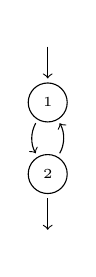
\begin{tikzpicture}
[
  every node/.style={
    font=\tiny
  },
  every initial by arrow/.style={
    shorten >=.5mm
  },
  every accepting by arrow/.style={
    shorten <=.5mm
  },
  entry above/.style={
    initial above,
    initial text=
  },
  exit below/.style={
    accepting below
  },
  bb/.style={
    circle,
    draw
  },
  tip/.style={
    shorten <=.5mm,
    shorten >=.5mm,
    ->,
    draw
  }
]

\node (entry) [bb,entry above] {$1$};
\node (body)  [bb,exit below,below=4mm of entry] {$2$};

\path [tip, bend right] (entry) edge (body);
\path [tip, bend right] (body) edge (entry);
\end{tikzpicture}

\end{block}

\column{.30\textwidth}
\begin{block}{\cinline{while} Loops}
\centering

% while-loop.tex: while loop shape.

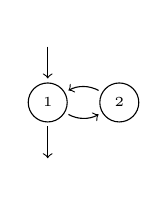
\begin{tikzpicture}
[
  every node/.style={
    font=\tiny
  },
  every initial by arrow/.style={
    shorten >=.5mm
  },
  every accepting by arrow/.style={
    shorten <=.5mm
  },
  entry above/.style={
    initial above,
    initial text=
  },
  exit below/.style={
    accepting below
  },
  bb/.style={
    circle,
    draw
  },
  tip/.style={
    shorten <=.5mm,
    shorten >=.5mm,
    ->,
    draw
  }
]

\node (entry) [bb,entry above,exit below] {$1$};
\node (body)  [bb,right=4mm of entry] {$2$};

\path [tip, bend right] (entry) edge (body);
\path [tip, bend right] (body) edge (entry);
\end{tikzpicture}

\end{block}

\column{.30\textwidth}
\begin{block}{Irreducible Loops}
\centering

% irreducible-loop.tex: irreducible loop shape.

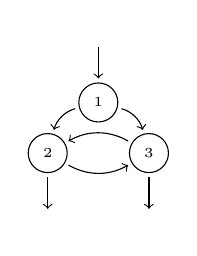
\begin{tikzpicture}
[
  every node/.style={
    font=\tiny
  },
  every initial by arrow/.style={
    shorten >=.5mm
  },
  every accepting by arrow/.style={
    shorten <=.5mm
  },
  entry above/.style={
    initial above,
    initial text=
  },
  exit below/.style={
    accepting below
  },
  bb/.style={
    circle,
    draw
  },
  tip/.style={
    shorten <=.5mm,
    shorten >=.5mm,
    ->,
    draw
  }
]

\node (entry)  [bb,entry above] {$1$};
\node (body-1) [bb,exit below,below left=4mm of entry] {$2$};
\node (body-2) [bb,exit below,below right=4mm of entry] {$3$};

\path [tip,bend right] (entry) edge (body-1);
\path [tip,bend left]  (entry) edge (body-2);

\path [tip,bend right] (body-1) edge (body-2);
\path [tip,bend right] (body-2) edge (body-1);
\end{tikzpicture}

\end{block}
\end{columns}

\bigskip
In LLVM the focus is on one kind of loop:

\begin{itemize}
\item natural loops
\end{itemize}
\end{frame}

\begin{frame}{Natural Loops}
A natural loop:

\begin{itemize}
\item has only one entry node -- \emph{header}
\item there is a back edge that enter the loop header
\end{itemize}

Under this definition:

\begin{itemize}
\item the irreducible loop is not a natural loop
\item since LLVM consider only natural loops, the irreducible loop \alert{is not
      recognized} as a loop
\end{itemize}
\end{frame}

\begin{frame}{Loop Terminology}
Loops defined starting from back-edges:

\begin{description}
\item[back-edge] edge entering loop header: $(3,1)$
\end{description}

\begin{columns}[t]
\column{.59\textwidth}
\begin{description}
\item[header] loop entry node: $1$
\item[body] nodes that can reach back-edge source node ($3$) without passing
            from back-edge target node ($1$) plus back-edge target node:
            $\{1 ,2, 3\}$
\end{description}
\column{.32\textwidth}
\vspace*{-1em}
\begin{block}{\small A loop}
\vspace*{-1em}

% loop-nodes.tex: loop terminology by picture.

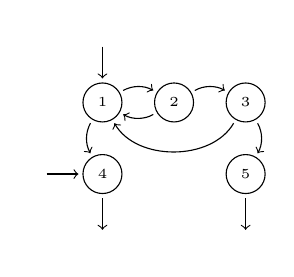
\begin{tikzpicture}
[
  every node/.style={
    font=\tiny
  },
  every initial by arrow/.style={
    shorten >=.5mm
  },
  every accepting by arrow/.style={
    shorten <=.5mm
  },
  entry above/.style={
    initial above,
    initial text=
  },
  entry left/.style={
    initial left,
    initial text=
  },
  exit below/.style={
    accepting below
  },
  bb/.style={
    circle,
    draw
  },
  tip/.style={
    shorten <=.5mm,
    shorten >=.5mm,
    ->,
    draw
  }
]

\node (entry)  [bb,entry above] {$1$};
\node (body-1) [bb,right=4mm of entry] {$2$};
\node (body-2) [bb,right=4mm of body-1] {$3$};

\node (exit-1) [bb,entry left,exit below,below=4mm of entry] {$4$};
\node (exit-2) [bb,exit below,below=4mm of body-2] {$5$};

\path [tip,bend left] (entry) edge (body-1);
\path [tip,bend left] (body-1) edge (body-2);

\path [tip,bend left]    (body-1) edge (entry);
\path [tip,bend left=60] (body-2) edge (entry);

\path [tip,bend right] (entry) edge (exit-1);
\path [tip,bend left]  (body-2) edge (exit-2);
\end{tikzpicture}

\end{block}


\end{columns}

\begin{description}
\item[exiting] nodes with a successor outside the loop: $\{1, 3\}$
\item[exit] nodes with a predecessor inside the loop: $\{4, 5\}$
\end{description}
\end{frame}

\begin{frame}{Loop Simplify}
Natural loops finding is the base pass \alert{identify} loops, but:

\begin{itemize}
\item some features are not analysis/optimization friendly
\end{itemize}

The \texttt{loop-simplify} pass normalize natural loops:

\begin{columns}[t]
\column{.50\textwidth}
\begin{description}
\item[pre-header] the \alert{only predecessor} of \alert{header} node
\item[latch] the \alert{starting node} of the \alert{only back-edge}
\item[exit-block] ensures \alert{exits dominated} by loop \alert{header}
\end{description}

\column{.40\textwidth}
\begin{block}{Pre-header Insertion}
\centering

% pre-header.tex: adding pre-header.

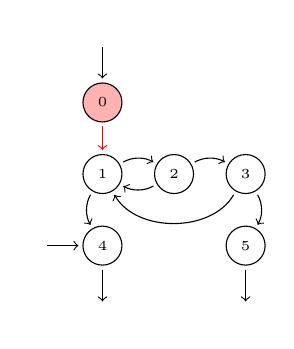
\begin{tikzpicture}
[
  every node/.style={
    font=\tiny
  },
  every initial by arrow/.style={
    shorten >=.5mm
  },
  every accepting by arrow/.style={
    shorten <=.5mm
  },
  entry above/.style={
    initial above,
    initial text=
  },
  entry left/.style={
    initial left,
    initial text=
  },
  exit below/.style={
    accepting below
  },
  bb/.style={
    circle,
    draw
  },
  tip/.style={
    shorten <=.5mm,
    shorten >=.5mm,
    ->,
    draw
  }
]

\node (pre-header) [bb,entry above,fill=red!30] {$0$};

\node (entry)  [bb,below=4mm of pre-header] {$1$};
\node (body-1) [bb,right=4mm of entry] {$2$};
\node (body-2) [bb,right=4mm of body-1] {$3$};

\node (exit-1) [bb,entry left,exit below,below=4mm of entry] {$4$};
\node (exit-2) [bb,exit below,below=4mm of body-2] {$5$};

\path [tip,color=red] (pre-header) edge (entry);

\path [tip,bend left] (entry) edge (body-1);
\path [tip,bend left] (body-1) edge (body-2);

\path [tip,bend left]    (body-1) edge (entry);
\path [tip,bend left=60] (body-2) edge (entry);

\path [tip,bend right] (entry) edge (exit-1);
\path [tip,bend left]  (body-2) edge (exit-2);
\end{tikzpicture}

\end{block}
\end{columns}
\end{frame}

\begin{frame}{Loop Simplify}{Example}
\begin{columns}[t]
\column{.45\textwidth}
\begin{block}{Latch Insertion}
\centering

% latch.tex: ensure only one back-edge.

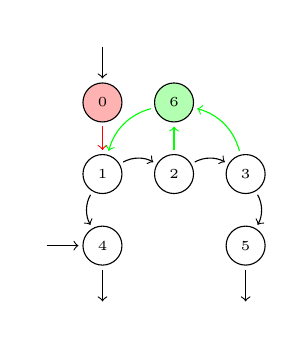
\begin{tikzpicture}
[
  every node/.style={
    font=\tiny
  },
  every initial by arrow/.style={
    shorten >=.5mm
  },
  every accepting by arrow/.style={
    shorten <=.5mm
  },
  entry above/.style={
    initial above,
    initial text=
  },
  entry left/.style={
    initial left,
    initial text=
  },
  exit below/.style={
    accepting below
  },
  bb/.style={
    circle,
    draw
  },
  tip/.style={
    shorten <=.5mm,
    shorten >=.5mm,
    ->,
    draw
  }
]

\node (pre-header) [bb,entry above,fill=red!30] {$0$};

\node (entry)  [bb,below=4mm of pre-header] {$1$};
\node (body-1) [bb,right=4mm of entry] {$2$};
\node (body-2) [bb,right=4mm of body-1] {$3$};
\node (latch)  [bb,above=4mm of body-1,fill=green!30] {$6$};

\node (exit-1) [bb,entry left,exit below,below=4mm of entry] {$4$};
\node (exit-2) [bb,exit below,below=4mm of body-2] {$5$};

\path [tip,color=red] (pre-header) edge (entry);

\path [tip,bend left] (entry) edge (body-1);
\path [tip,bend left] (body-1) edge (body-2);

\path [tip,color=green]            (body-1) edge (latch);
\path [tip,color=green,bend right] (body-2) edge (latch);
\path [tip,color=green,bend right] (latch) edge (entry);

\path [tip,bend right] (entry) edge (exit-1);
\path [tip,bend left]  (body-2) edge (exit-2);
\end{tikzpicture}

\end{block}

\column{.45\textwidth}
\begin{block}{Exit-block Insertion}
\centering

% exit-block.tex: ensure loop exit dominated by loop header.

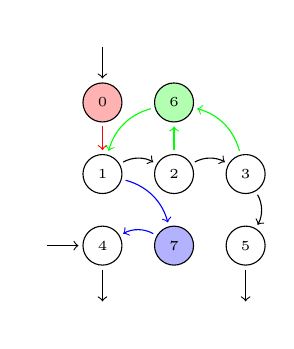
\begin{tikzpicture}
[
  every node/.style={
    font=\tiny
  },
  every initial by arrow/.style={
    shorten >=.5mm
  },
  every accepting by arrow/.style={
    shorten <=.5mm
  },
  entry above/.style={
    initial above,
    initial text=
  },
  entry left/.style={
    initial left,
    initial text=
  },
  exit below/.style={
    accepting below
  },
  bb/.style={
    circle,
    draw
  },
  tip/.style={
    shorten <=.5mm,
    shorten >=.5mm,
    ->,
    draw
  }
]

\node (pre-header) [bb,entry above,fill=red!30] {$0$};

\node (entry)  [bb,below=4mm of pre-header] {$1$};
\node (body-1) [bb,right=4mm of entry] {$2$};
\node (body-2) [bb,right=4mm of body-1] {$3$};
\node (latch)  [bb,above=4mm of body-1,fill=green!30] {$6$};

\node (exit-0) [bb,below=4mm of body-1,fill=blue!30] {$7$};
\node (exit-1) [bb,entry left,exit below,below=4mm of entry] {$4$};
\node (exit-2) [bb,exit below,below=4mm of body-2] {$5$};

\path [tip,color=red] (pre-header) edge (entry);

\path [tip,bend left] (entry) edge (body-1);
\path [tip,bend left] (body-1) edge (body-2);

\path [tip,color=green]            (body-1) edge (latch);
\path [tip,color=green,bend right] (body-2) edge (latch);
\path [tip,color=green,bend right] (latch) edge (entry);

\path [tip,bend left,color=blue]  (entry) edge (exit-0);
\path [tip,bend right,color=blue] (exit-0) edge (exit-1);
\path [tip,bend left]             (body-2) edge (exit-2);
\end{tikzpicture}

\end{block}
\end{columns}

\begin{itemize}
\item pre-header always executed before entering the loop
\item latch always executed before starting a new iteration
\item exit-blocks always executed after exiting the loop
\end{itemize}
\end{frame}

\begin{frame}{Loop-closed SSA}
Loop representation can be further normalized:

\begin{itemize}
\item \texttt{loop-simplify} normalize the \alert{shape} of the loop
\item nothing is said about loop definitions
\end{itemize}

Keeping SSA form is expensive with loops:

\begin{itemize}
\item \texttt{lcssa} insert \llvminline{phi} instruction at loop boundaries for
      variables \alert{defined inside} the loop body and \alert{used outside}
\item this guarantee isolation between optimization performed inside and outside
      the loop
\item faster keeping IR into SSA form -- propagation of code changes outside the
      loop blocked by \llvminline{phi} instructions
\end{itemize}
\end{frame}

\begin{frame}{Loop-closed SSA}{Example}
\begin{block}{Linear Search}
\centering
\cinput{snippet/02/lcssa.c}
\end{block}

The example is trivial:

\begin{itemize}
\item think about having large loop bodies
\item transformation becomes useful
\end{itemize}
\end{frame}

\begin{frame}{Loop-closed SSA}{Example}
\begin{block}{Before LCSSA}
\centering
\llvminput{snippet/02/before-lcssa.ll}
\end{block}
\end{frame}

\begin{frame}{Loop-closed SSA}{Example}
\begin{block}{After LCSSA}
\centering
\llvminput{snippet/02/after-lcssa.ll}
\end{block}
\end{frame}

\begin{frame}{Induction Variables}
Some loop variables are \emph{special}:

\begin{itemize}
\item e.g. counters
\end{itemize}

Generalization lead to \alert{induction variables}:

\begin{itemize}
\item \cinline{foo} is a loop induction variable if its successive values form
      an arithmetic progression:

      \begin{center}
      \cinline{foo = bar * baz + biz}
      \end{center}

      where \cinline{bar, biz} are
      loop-invariant~\footnote{Constants inside the loop}, and \cinline{baz} is
      an induction variable
\item \cinline{foo} is a \alert{canonical} induction variable if it is always
      incremented by a constant amount:

      \begin{center}
      \cinline{foo = foo + biz}
      \end{center}

      where \cinline{biz} is loop-invariant
\end{itemize}
\end{frame}

\begin{frame}{Induction Variable Simplification}
Canonical induction variables are used to \alert{drive} loop execution:

\begin{itemize}
\item given a loop, the \texttt{indvars} pass tries to find its canonical
      induction variable
\end{itemize}

With respect to theory, LLVM canonical induction variable is:

\begin{itemize}
\item initialized to \llvminline{0}
\item incremented by \llvminline{1} at each loop iteration
\end{itemize}
\end{frame}

\begin{frame}{Normalization}{Wrap-up}
Normalization passes running order:

\begin{enumerate}
\item \texttt{mem2reg}: limit use of memory, increasing the effectiveness of
       subsequent passes
\item \texttt{loop-simplify}: canonicalize loop shape, lower burden of writing
      passes
\item \texttt{lcssa}: keep effects of subsequent loop optimizations local,
      limiting overhead of maintaining SSA form
\item \texttt{indvars}: normalize induction variables, highlighting the
      canonical induction variable
\end{enumerate}

Other normalization passes available:

\begin{itemize}
\item try running \texttt{opt -help}
\end{itemize}
\end{frame}



\section{Analysis Passes}
\begin{frame}{Checking Input Properties}
Analysis basically allows to:

\begin{itemize}
\item \alert{derive} information and properties of the input
\item \alert{verify} properties of input
\end{itemize}

Keeping analysis information is expensive:

\begin{itemize}
\item tuned algorithms updates analysis information when an optimization
      invalidates them
\item incrementally updating analysis is cheaper than recomputing them
\end{itemize}

Many LLVM analysis supports incremental updates:

\begin{itemize}
\item this is an \alert{optimization}
\item forget this feature for the home-work
\item focus on \alert{information} provided by analysis
\end{itemize}
\end{frame}

\begin{frame}{Useful Analysis}
We will see the following passes:

\begin{block}{Analysis}
\centering
\begin{tabular}{ccc}
\toprule

\multicolumn{1}{c}{\textbf{Pass}}        &
\multicolumn{1}{c}{\textbf{Switch}}      &
\multicolumn{1}{c}{\textbf{Transitive}} \\

\midrule

Control flow graph  &
\texttt{none}       &
No                 \\

Dominator tree    &
\texttt{domtree}  &
No               \\

Post-dominator tree   &
\texttt{postdomtree}  &
No                   \\

Loop information  &
\texttt{loops}    &
Yes              \\

Scalar evolution           &
\texttt{scalar-evolution}  &
Yes                       \\

Alias analysis    &
\texttt{special}  &
Yes              \\

Memory dependence  &
\texttt{memdep}    &
Yes               \\

\bottomrule
\end{tabular}
\end{block}

Requiring analysis by transitivity:

\begin{description}
\item[yes] \cppinline{llvm::AnalysisUsage::addRequiredTransitive<T>()}
\item[no] \cppinline{llvm::AnalysisUsage::addRequired<T>()}
\end{description}
\end{frame}

\begin{frame}{Control Flow Graph}
The Control Flow Graph is implicitly maintained by LLVM:

\begin{itemize}
\item no specific pass to build it
\end{itemize}

Recap:

\begin{itemize}
\item CFG for a function is a set of basic blocks
\item a basic block is a set of instructions
\end{itemize}

Functions and basic blocks acts like containers:

\begin{itemize}
\item STL-like accessors: \cppinline{front()}, \cppinline{back()},
      \cppinline{size()}, \ldots
\item STL-like iterators: \cppinline{begin()}, \cppinline{end()}
\end{itemize}

Each contained element is aware of its container:

\begin{itemize}
\item \cppinline{getParent()}
\end{itemize}
\end{frame}

\begin{frame}{Control Flow Graph}{Walking}
Every CFG has an entry basic block:

\begin{itemize}
\item the \alert{first} executed basic block
\item it is the \alert{root/source} of the graph
\item get it with \cppinline{llvm::Function::getEntryBlock()}
\end{itemize}

More than one exit blocks can be generated:

\begin{itemize}
\item their terminator instructions are \llvminline{ret}s
\item they are the \alert{leaves/sinks} of the graph
\item use \cppinline{llvm::BasicBlock::getTerminator()} to get the terminator
      \ldots
\item \ldots then check its real class
\end{itemize}
\end{frame}

\begin{frame}{Side Note}{Casting Framework}
For performance reasons, a custom casting framework is used:

\begin{itemize}
\item you cannot use \cppinline{static\_cast} and \cppinline{dynamic\_cast} with
      types/classes provided by LLVM
\end{itemize}

\begin{block}{LLVM Casting Functions}
\centering
\begin{tabular}{cc}
\toprule

\multicolumn{1}{c}{\textbf{Meaning}}   &
\multicolumn{1}{c}{\textbf{Function}} \\

\midrule

Static cast of \cppinline{Y *} to \cppinline{X *}  &
\cppinline{X * llvm::cast<X>(Y *)}                \\

Dynamic cast of \cppinline{Y *} to \cppinline{X *}  &
\cppinline{X * llvm::dyn\_cast<X>(Y *)}            \\

Is \cppinline{Y} an \cppinline{X}?  &
\cppinline{bool llvm::isa<X>(Y *)} \\

\bottomrule
\end{tabular}
\end{block}

Example:

\begin{itemize}
\item is \cppinline{BB} a sink?
      \begin{center}
      \cppinline{llvm::isa<llvm::ReturnInst>(BB.getTerminator())}
      \end{center}
\end{itemize}
\end{frame}

\begin{frame}{Control Flow Graph}{Basic Blocks}
Every basic block \cppinline{BB} has one or more:

\begin{description}
\item[predecessors] from \cppinline{pred\_begin(BB)} to
      \cppinline{pred\_end(BB)} \footnote{see include/llvm/IR/CFG.h}
\item[successors] from \cppinline{succ\_begin(BB)} to
      \cppinline{succ\_end(BB)}
\end{description}

Convenience accessors directly available in \cppinline{llvm::BasicBlock}:

\begin{itemize}
\item e.g. \cppinline{llvm::BasicBlock::getUniquePredecessor()}
\end{itemize}

Other convenience member functions:

\begin{itemize}
\item moving a basic block:
      \cppinline{llvm::BasicBlock::moveBefore(llvm::BasicBlock *)} or
      \cppinline{llvm::BasicBlock::moveAfter(llvm::BasicBlock *)}
\item split a basic block:
      \cppinline{llvm::BasicBlock::splitBasicBlock(llvm::BasicBlock::iterator)}
\item \ldots
\end{itemize}
\end{frame}

\begin{frame}{Control Flow Graph}{Instructions}
The \cppinline{llvm::Instruction} class define common operations:

\begin{itemize}
\item e.g. getting an operand: \cppinline{llvm::Instruction::getOperand(unsigned)}
\end{itemize}

Subclasses provide specialized accessors:

\begin{itemize}
\item e.g the \llvminline{load} instruction takes an operand that is a pointer:
      \cppinline{llvm::LoadInst::getPointerOperand()}
\end{itemize}

The value produced by the instruction is the \alert{instruction itself}:

\begin{block}{Example}
Consider:

\centering
\llvminline{\%6 = load i32, i32* \%1, align 4}

\flushleft
the \llvminline{load} is described
by an instance of \cppinline{llvm::LoadInst}. That instance also models the
\llvminline{\%6} variable
\end{block}
\end{frame}

\begin{frame}{Instructions}{Creating New Instructions}
Instructions built using:

\begin{itemize}
\item constructors -- e.g. \cppinline{llvm::LoadInst::LoadInst(...)}
\item factory methods -- e.g. \cppinline{llvm::GetElementPtrInst::Create(...)}
\end{itemize}

Interface is not homogeneous:

\begin{itemize}
\item some instructions support both methods
\item others support only one
\end{itemize}

At build-time, instructions can be:

\begin{itemize}
\item appended to a basic block
\item inserted after/before a given instruction
\end{itemize}

Insertion point usually specified as builder last argument
\end{frame}

\begin{frame}{Side Note}{Definitions and Uses}
LLVM class hierarchy is built around two simple concepts:

\begin{description}
\item[value] something that can be used: \cppinline{llvm::Value}
\item[user] something that can use: \cppinline{llvm::User}
\end{description}

A value is a \alert{definition}:

\begin{itemize}
\item \cppinline{llvm::Value::use\_begin()},
      \cppinline{llvm::Value::use\_end()} to visit uses
      \footnote{\cppinline{llvm::Instruction} derives from \cppinline{llvm::Value}}
\end{itemize}

An user access \alert{definitions}:

\begin{itemize}
\item \cppinline{llvm::User::op\_begin()},
      \cppinline{llvm::User::op\_end()} to visit used values
      \footnote{\cppinline{llvm::Value} derives from \cppinline{llvm::User}}
\end{itemize}

\begin{columns}[t]
\column{.45\textwidth}
Functions:

\begin{itemize}
\item used by call sites
\item uses formal parameters
\end{itemize}

\column{.45\textwidth}
Instructions:

\begin{itemize}
\item define an SSA value
\item uses operands
\end{itemize}
\end{columns}
\end{frame}

\begin{frame}{Side Note}{Value Typing}
Every \cppinline{llvm::Value} is typed:

\begin{itemize}
\item use \cppinline{llvm::Value::getType()} to get the type
\end{itemize}

Since every instructions is/define a value:

\begin{itemize}
\item instructions are typed
\end{itemize}

\begin{block}{Example}
Consider:

\centering
\llvminline{\%6 = load i32, i32* \%1, align 4}

\flushleft
the \llvminline{\%6} variable actually is the instruction itself. Its type is
the type of \llvminline{load} return value, \llvminline{i32}
\end{block}
\end{frame}

\begin{frame}{Dominance Trees}
Dominance trees answer to control-related queries:

\begin{columns}[t]
\column{.45\textwidth}
\begin{itemize}
\item is this basic block executed before that?
\item \cppinline{llvm::DominatorTree}
\end{itemize}

\column{.45\textwidth}
\begin{itemize}
\item is this basic block executed after that?
\item \cppinline{llvm::PostDominatorTree}
\end{itemize}
\end{columns}

\bigskip
The two trees interface is similar:

\begin{itemize}
\item \cppinline{bool dominates(X *, X *)}
\item \cppinline{bool properlyDominates(X *, X *)}
\end{itemize}

Where \cppinline{X} is an \cppinline{llvm::BasicBlock} or an
\cppinline{llvm::Instruction}

\bigskip
Using \texttt{opt} is possible printing them:

\begin{itemize}
\item \texttt{-view-dom}, \texttt{-dot-dom}
\item \texttt{-view-postdom}, \texttt{-dot-postdom}
\end{itemize}
\end{frame}

\begin{frame}{Loop Information}
Loop information are represented using two classes:

\begin{itemize}
\item \cppinline{llvm::LoopInfo} analysis detects natural loops
\item \cppinline{llvm::Loop} represents a single loop
\end{itemize}

Using \cppinline{llvm::LoopInfo} it is possible:

\begin{itemize}
\item navigate through top-level loops: \\
      \cppinline{llvm::LoopInfo::begin()}, \cppinline{llvm::LoopInfo::end()}
\item get the loop for a given basic block: \\
      \cppinline{llvm::LoopInfo::operator[](llvm::BasicBlock *)}
\end{itemize}
\end{frame}

\begin{frame}{Loop Information}{Nesting Tree}
Loops are represented in a \alert{nesting tree}:

\begin{columns}[t]
\column{.45\textwidth}
\begin{block}{Source}
\centering
\cinput{snippet/02/loop-nest.c}
\end{block}

\column{.45\textwidth}
\begin{block}{Loop Nest}
\centering

% loop-nest.tex: a simple loop nest.

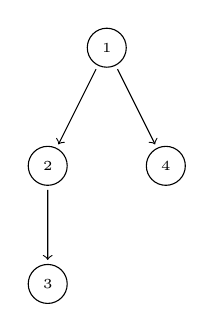
\begin{tikzpicture}
[
  every node/.style={
    font=\tiny
  },
  loop/.style={
    circle,
    draw
  },
  tip/.style={
    shorten <=.5mm,
    shorten >=.5mm,
    ->,
    draw
  },
  level 1/.style={
    edge from parent/.style=tip
  },
]

\node [loop] {$1$}
  child { node [loop] {$2$}
    child { node [loop] {$3$}}
  }
  child { node [loop] {$4$}};
\end{tikzpicture}

\end{block}
\end{columns}

Nest navigation:

\begin{itemize}
\item children loops: \cppinline{llvm::Loop::begin()},
      \cppinline{llvm::Loop::end()}
\item parent loop: \cppinline{llvm::Loop::getParentLoop()}
\end{itemize}
\end{frame}

\begin{frame}{Loop Information}{Query Loops}
Accessors for relevant nodes also available:

\begin{description}
\item[pre-header] \cppinline{llvm::Loop:getLoopPreheader()}
\item[header] \cppinline{llvm::Loop::getHeader()}
\item[latch] \cppinline{llvm::Loop::getLoopLatch()}
\item[exiting] \cppinline{llvm::Loop::getLoopExiting()}, \\
               \cppinline{llvm::Loop::getExitingBlocks(...)}
\item[exit] \cppinline{llvm::Loop::getExitBlock()} \\
            \cppinline{llvm::Loop::getExitBlocks(...)}
\end{description}

Loop basic blocks accessible via:

\begin{description}
\item[iterators] \cppinline{llvm::Loop::block\_begin()}, \\
                 \cppinline{llvm::Loop::block\_end()}
\item[vector]
      \cppinline{std::vector<llvm::BasicBlock *> \&llvm::Loop::getBlocks()}
\end{description}
\end{frame}

\begin{frame}{Scalar Evolution}
The \alert{SC}alar \alert{EV}olution framework:

\begin{itemize}
\item represents scalar expressions
\item supports recursive updates
\item lower burden of explicitly handling expressions composition
\item is designed to support \alert{general induction variables}
\end{itemize}

\begin{columns}\column{.64\textwidth}
\begin{block}{Example}
\centering
\llvminput{snippet/02/basic-scev.ll}
\end{block}

\column{.30\textwidth}
SCEV for \llvminline{\%i.0}:

\begin{itemize}
\item initial value $0$
\item incremented
\item by $1$ at each iteration
\item final value $10$
\end{itemize}
\end{columns}
\end{frame}

\begin{frame}{Scalar Evolution}{Example}
\begin{columns}
\column{.55\textwidth}
\begin{block}{Source}
\centering
\cinput{snippet/02/nested-scev.c}
\end{block}

\column{.35\textwidth}
SCEV \llvminline{\{A,B,C\}<\%D>}:

\begin{itemize}
\item \llvminline{A} initial
\item \llvminline{B} operator
\item \llvminline{C} operand
\item \llvminline{D} defining BB
\end{itemize}
\end{columns}

\begin{block}{Induction Variables}
\centering
\llvminput{snippet/02/nested-scev-induction.ll}
\end{block}
\end{frame}

\begin{frame}{Scalar Evolution}{More than Induction Variables}
The scalar evolution framework manages \alert{any scalar expression}:

\begin{block}{Pointer SCEVs}
\centering
\llvminput{snippet/02/nested-scev-pointer.ll}
\end{block}

SCEV is an analysis used for common optimizations:

\begin{itemize}
\item induction variable substitution
\item strength reduction
\item vectorization
\item \ldots
\end{itemize}
\end{frame}

\begin{frame}{Scalar Evolution}{SCEVs Design}
SCEVs are modeled by the \cppinline{llvm::SCEV} class:

\begin{itemize}
\item a subclass for each kind of SCEV: e.g. \cppinline{llvm::SCEVAddExpr}
\item instantiation disabled
\end{itemize}

A SCEV actually is a tree of SCEVs:

\begin{itemize}
\item \llvminline{\{(80 + \%bar),+,80\}} = \llvminline{\{\%1,+,80\}},
      \llvminline{\%1 = 80 + \%bar}
\end{itemize}

Tree leaves:

\begin{description}
\item[constant] \cppinline{llvm::SCEVConstant}: e.g. \llvminline{80}
\item[unknown~\footnote{Not further splittable}] \cppinline{llvm::SCEVUnknown}:
                                                 e.g. \llvminline{\%bar}
\end{description}

SCEV tree explorable through the visitor pattern:

\begin{itemize}
\item \cppinline{llvm::SCEVVisitor}
\end{itemize}
\end{frame}

\begin{frame}{Scalar Evolution}{Analysis Interface}

The \cppinline{llvm::ScalarEvolution} class:

\begin{itemize}
\item analyzes SCEVs for a \cppinline{llvm::Function}
\item builds SCEVs for values: \\
      \cppinline{llvm::ScalarEvolution::getSCEV(llvm::Value *)}
\item creates new SCEVs: \\
% It looks horrible, but I must do that to take line length < of 80 chars.
\cppinline{llvm::ScalarEvolution::getConstant(llvm::ConstantInt *)} \\
\cppinline{llvm::ScalarEvolution::getAddExpr(llvm::SCEV *, llvm::SCEV *)} \\
\ldots
\item gets important SCEVs: \\
      \cppinline{llvm::ScalarEvolution::getBackedgeTakenCount(llvm::Loop *)} \\
      \cppinline{llvm::ScalarEvolution::getPointerBase(llvm::SCEV *)} \\
      \ldots
\end{itemize}
\end{frame}

\begin{frame}{Alias Analysis}
Let $X$ be an instruction accessing a memory location:

\begin{itemize}
\item is there another instruction accessing the same location?
\end{itemize}

Alias analysis tries to answer the question:

\begin{description}
\item[application] memory operation scheduling
\item[problem] often fails
\end{description}

Different algorithms for alias analysis:

\begin{itemize}
\item common interface -- \cppinline{llvm::AliasAnalysis} -- for all algorithms
\item by default, basic alias analyzer -- \texttt{basicaa} -- is used
\end{itemize}

\begin{block}{Requiring Alias Analysis}
\centering
\cppinput{snippet/02/requiring-alias-analysis.cpp}
\end{block}
\end{frame}

\begin{frame}{Alias Analysis}{Memory Representation}
\begin{columns}[t]
\column{.45\textwidth}
\begin{block}{Source}
\centering
\llvminput{snippet/02/memory-locations.ll}
\end{block}

\column{.45\textwidth}
\begin{block}{Distinct Locations}
\centering

% alias-analysis-distinct.tex: different locations.

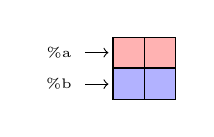
\begin{tikzpicture}
[
  every node/.style={
    font=\tiny
  },
  location/.style={
    rectangle split,
    rectangle split parts=2,
    rotate=90,
    draw
  },
  location-a/.style={
    location,
    rectangle split part fill={
      red!30,
      red!30
    }
  },
  location-b/.style={
    location,
    rectangle split part fill={
      blue!30,
      blue!30
    }
  },
  tip/.style={
    shorten <=.5mm,
    shorten >=.5mm,
    ->,
    draw
  }
]

\matrix [column sep=4mm]
{
\node (a) {\llvminline{\%a}}; & \node (a-loc) [location-a] {}; \\
\node (b) {\llvminline{\%b}}; & \node (b-loc) [location-b] {}; \\
};

\path [tip] (a) edge (a-loc.north);
\path [tip] (b) edge (b-loc.north);
\end{tikzpicture}

\end{block}
\end{columns}

\begin{columns}[t]
\column{.45\textwidth}
\begin{block}{Same Location}
\centering

% alias-analysis-same.tex: same location.

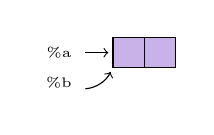
\begin{tikzpicture}
[
  every node/.style={
    font=\tiny
  },
  location/.style={
    rectangle split,
    rectangle split parts=2,
    rectangle split part fill={
      red!30!blue!30,
      red!30!blue!30
    },
    rotate=90,
    draw
  },
  tip/.style={
    shorten <=.5mm,
    shorten >=.5mm,
    ->,
    draw
  }
]

\matrix [column sep=4mm]
{
\node (a) {\llvminline{\%a}}; & \node (loc) [location] {}; \\
\node (b) {\llvminline{\%b}}; &                            \\
};

\path [tip]            (a) edge (loc.north);
\path [tip,bend right] (b) edge (loc.north west);
\end{tikzpicture}

\end{block}

\column{.45\textwidth}
\begin{block}{Overlapping Locations}
\centering

% alias-analysis-overlapping.tex: overlapping locations.

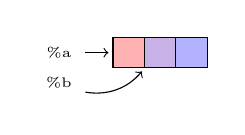
\begin{tikzpicture}
[
  every node/.style={
    font=\tiny
  },
  location/.style={
    rectangle split,
    rectangle split parts=3,
    rectangle split part fill={
      red!30,
      red!30!blue!30,
      blue!30
    },
    rotate=90,
    draw
  },
  tip/.style={
    shorten <=.5mm,
    shorten >=.5mm,
    ->,
    draw
  }
]

\matrix [column sep=4mm]
{
\node (a) {\llvminline{\%a}}; & \node (loc) [location] {}; \\
\node (b) {\llvminline{\%b}}; &                            \\
};

\path [tip]           (a) edge (loc.north);
\path [tip,bend right] (b) edge (loc.text split west);
\end{tikzpicture}

\end{block}
\end{columns}

\bigskip
Basic building block is \cppinline{llvm::AliasAnalysis::Location}:

\begin{itemize}
\item address: e.g. \llvminline{\%a}
\item size: e.g. 2 bytes
\end{itemize}
\end{frame}

\begin{frame}{Alias Analyzer}{Basic Interface}
Given two locations $X$, $Y$, the alias analyzer classifies them:

\begin{itemize}
\item \cppinline{llvm::AliasAnalyzer::NoAlias}: $X$ and $Y$ are different
      memory locations
\item \cppinline{llvm::AliasAnalyzer::MustAlias}: $X$ and $Y$ are equal -- i.e.
      they points to the same address
\item \cppinline{llvm::AliasAnalyzer::PartialAlias}: $X$ and $Y$ partially
      overlap -- i.e. they points to different addresses, but the pointed memory
      areas partially overlap
\item \cppinline{llvm::AliasAnalyzer::MayAlias}: unable to compute aliasing
      information -- i.e. $X$ and $Y$ can be different locations, or $X$ can be
      a complete/partial alias of $Y$
\end{itemize}

Queries performed using:

\begin{itemize}
\item \cppinline{llvm::AliasAnalyzer::alias(X, Y)}
\end{itemize}
\end{frame}

\begin{frame}{Alias Analyzer}{Mid-level Interface}
Basic alias analyzer interface is low-level -- we would like expressing queries
about a single pointer $X$:

\begin{itemize}
\item how referenced memory location is accessed?
\item which other instructions reference the same location?
\end{itemize}

What we need is a set, to classify memory locations:

\begin{itemize}
\item construct a \cppinline{llvm::AliasSetTracker} starting from a
      \cppinline{llvm::AliasAnalyer *}
\item it builds \cppinline{llvm::AliasSet}s
\end{itemize}

For a given location $X$, a \cppinline{llvm::AliasSet}:

\begin{itemize}
\item contains all locations aliasing with $X$
\end{itemize}
\end{frame}

\begin{frame}{Alias Analyzer}{Alias Set Memory Accesses}
Each alias set \alert{references} the memory:

\begin{itemize}
\item \cppinline{llvm::AliasSet::NoModRef}: no memory reference -- i.e. the set
      is empty
\item \cppinline{llvm::AliasSet::Mod}: memory accessed in write-mode -- e.g. a
      \llvminline{store} is inside the set
\item \cppinline{llvm::AliasSet::Ref}: memory accessed in read-mode -- e.g. a
      \llvminline{load} is inside the set
\item \cppinline{llvm::AliasSet::ModRef}: memory accessed in read-write mode --
      e.g. a \llvminline{load} and a \llvminline{store} inside the set
\end{itemize}
\end{frame}

\begin{frame}{Alias Analyzer}{Mid-level Interface}
Entry point is \cppinline{llvm::AliasSetTracker::getAliasSetForPointer(...)}:

\begin{itemize}
\item \cppinline{llvm::Value *}: location address
\item \cppinline{uint64\_t}: location size
\item \cppinline{llvm::MDNode *}: used for type-based alias
      analysis~\footnote{set to \cppinline{NULL}}
\item \cppinline{bool *}: whether a new \cppinline{llvm::AliasSet} has been
      created to hold the location -- location does not alias up to now
\end{itemize}

Having the \cppinline{llvm::AliasSet}:

\begin{itemize}
\item STL container-like interface: \cppinline{size()}, \cppinline{begin()},
      \cppinline{end()}, \ldots
\item check reference type: \cppinline{llvm::AliasSet::isRef()}, \ldots
\item check aliasing type: \cppinline{llvm::AliasSet::isMustAlias()}, \ldots
\end{itemize}
\end{frame}

\begin{frame}{Memory Dependence Analysis}{Alias Analyzer High-level Interface}
The \cppinline{llvm::MemoryDependenceAnalysis} wraps alias analysis to answer
queries in the following form:

\begin{itemize}
\item let \llvminline{\%foo} be an instruction accessing memory. Which
      preceding instructions does \llvminline{\%foo} depends on?
\end{itemize}

\begin{columns}[t]
\column{.45\textwidth}
Reads:

\begin{itemize}
\item \llvminline{store}s writing memory locations aliases with the one
      references by \llvminline{\%foo}
\end{itemize}

\column{.45\textwidth}
Writes:

\begin{itemize}
\item \llvminline{load}s reading memory locations aliased with the one
      referenced by \llvminline{\%foo}
\end{itemize}
\end{columns}
\end{frame}

\begin{frame}{Memory Dependence Analysis}{APIs}
Let \llvminline{\%foo} be a \cppinline{llvm::Instruction} accessing memory:

\begin{itemize}
\item call \cppinline{llvm::MemoryDependenceAnalysis::getDependency(...)}
\item you get a \llvminline{llvm::MemDepResult}
\end{itemize}

Dependencies are classified:

\begin{itemize}
\item \llvminline{llvm::MemDepResult::isClobber()}: an instruction clobbering --
      i.e. potentially modifying -- location referenced by \llvminline{\%foo}
      has been found
\item \llvminline{llvm::MemDepResult::isDef()}: an instruction defining -- e.g.
      writing -- the exact location referenced by \llvminline{\%foo} has been
      found
\item \llvminline{llvm::MemDepResult::isNonLocal()}: no dependency found on
      \llvminline{\%foo} basic block
\item \llvminline{llvm::MemDepResult::isNonFuncLocal()}: no dependency found on
      \llvminline{\%foo} function
\end{itemize}
\end{frame}

\section{Conclusions}
\begin{frame}{Conclusions}
Inside LLVM there a lot of passes:

\begin{description}
\item[normalization] put program into a canonical form
\item[analysis] get info about program
\end{description}

Please remember that

\begin{itemize}
\item a good compiler writer \alert{re-uses} code
\item check LLVM sources before re-implementing a pass
\end{itemize}
\end{frame}

\section{Bibliography}
\begin{frame}[allowframebreaks]{Bibliography}
\nocite{*}
\bibliographystyle{unsrt}
\bibliography{bibliography-2}
\end{frame}
\end{document}
